\section{工厂生产计划扩展(问题二)} % (fold)
\label{sec:工厂生产计划扩展}

现实情况中,新采购的组件并不能直接投入使用,而是应由供应商生产、交付、转运至库存中,再供生产取用。
因此,在生产工厂发出采购订单后,订购的组件需经过一定延迟时间,才能供实际生产使用。

\subsection{模型的建立与求解} % (fold)
\label{sub:模型的建立与求解}

% subsection 模型的建立与求解 (end)

本题要求在记入组件入库延迟的前提下,设计生产工厂每周7天的生产计划。
与问题一组件入库无延迟不同,问题二中组装产品所需的组件要提前一天入库才能参与生产。

在此基础上,由于该工厂第一天(周一)开始时没有任何组件库存,而新采购的组件在第二天(周二)才能投入生产,在第三天(周三)才可生产出WPCR。因此工厂必须在前一天(上周周日),准备好了刚好满足周一需求的WPCR库存(即$y_0^{\text{WPCR}} = 39+36=85$),以免缺货断供。

综上,本文在问题一模型基础上,添加以下约束条件:
\begin{equation}\label{新条件}
	\eta_{r^{\prime}}^{r} x_{t}^{r^{\prime}} \leqslant y_{t-1}^{r},\quad t=1,2, \cdots, T, r=1,2, \cdots, R.
\end{equation}
上式中,通过令工厂当天生产所需组件数量$\eta_{r^{\prime}}^{r} x_{t}^{r^{\prime}}$,小于前一天库存组件$y_{t-1}^{r}$,以限制工厂只得使用前一天的组件库存生产新组件。

将上式\ref{新条件}加入问题一中线性规划模型式\ref{总模型},得:

\begin{equation}\label{二模型}
	\begin{aligned}
&\min \quad z  = \sum_{t  = 1}^{T} \sum_{r = 1}^{R}\left(s^{r} \omega_{t}^{r}+h^{r} y_{t}^{r}\right)\\
& \ \begin{array}{r@{\quad}l@{}l@{\quad}l}
\mathrm{s.t. } 	&\sum_{r=1}^{R} M_{t}^{r} \leqslant M_{t}; &\\
&M_{t}^{r} \leqslant M_{t}^{r} \omega_{t}^{r}, &t=1,2, \cdots, T, r=1,2, \cdots, R;\\
& y_{t}^{r}=y_{t-1}^{r}+x_{t}^{r}-\eta_{r}^{r} x_{t}^{r^{\prime}}, &t=1,2, \cdots, T,  r=1,2, \cdots, R; \\
&\omega_{t}^{r} \in\{0,1\}, &t=1,2, \cdots, T, r=1,2, \cdots, R; \\
&x_{t}^{r}=x_{t}^{r} \omega_{t}^{r},&t=1,2, \cdots, T, r=1,2, \cdots, R;\\
&c^{r} x_{t}^{r}=M_{t}^{r} \omega_{t}^{r}, &t=1,2, \cdots, T, r=1,2, \cdots, R; \\
&M_{t}^{r} \geqslant 0,& r=1,2, \cdots, R ;\\
&y_{0}^{r}=y_{T}^{r}=0,& r=1,2, \cdots, R ;\\
&x_{t}^{r}, y_{t}^{r} \geqslant 0, &t=1,2, \cdots, T, r=1,2, \cdots, R;\\
&y_{t-1}^{\mathrm{WPCR}}+x_{t}^{\mathrm{WPCR}}-y_{t}^{\mathrm{WPCR}}=d_{t}, & t=1,2, \cdots, T; \\
&\eta_{r^{\prime}}^{r} x_{t}^{r^{\prime}} \leqslant y_{t-1}^{r}, &t=1,2, \cdots, T, r=1,2, \cdots, R;
\end{array}.
\end{aligned}
\end{equation}

\subsection{生产方案展示} % (fold)
\label{sub:生产方案展示}

\begin{figure}[!htbp]
	\centering
	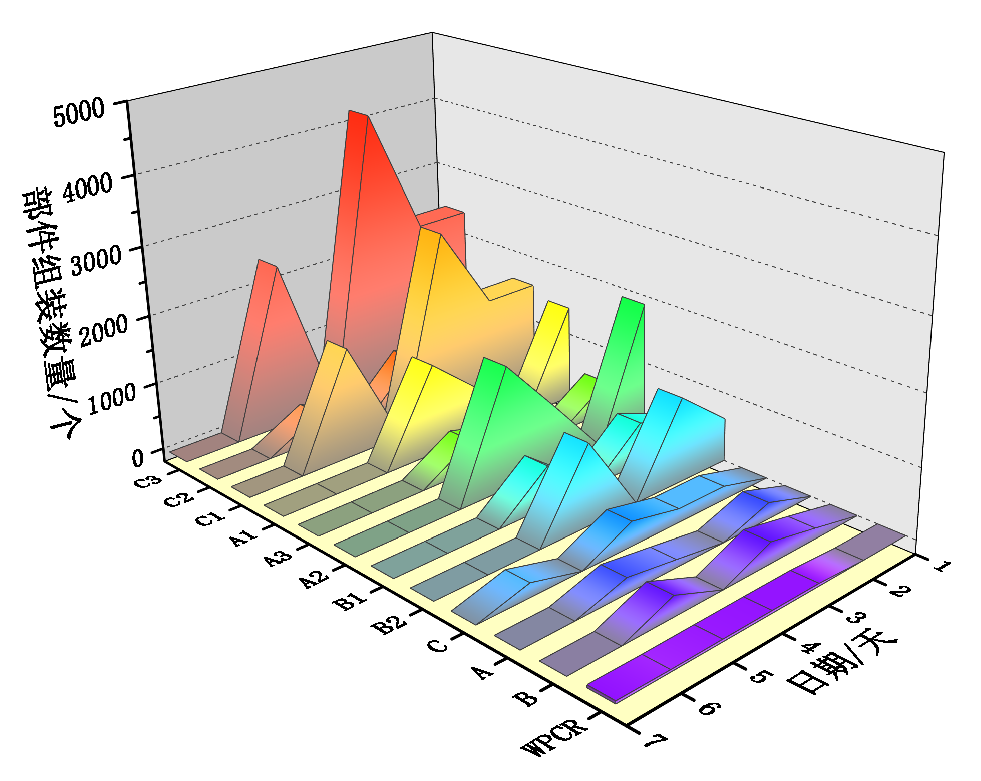
\includegraphics{Image/问题二展示.eps}
	\caption{问题二}\label{问题二}
\end{figure}

\begin{figure}[!htbp]
	\centering
	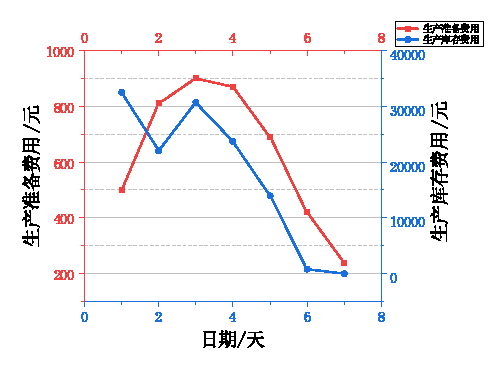
\includegraphics{Image/问题二展示2.eps}
	\caption{问题二2}\label{问题二2}
\end{figure}

\begin{figure}[!htbp]
	\centering
	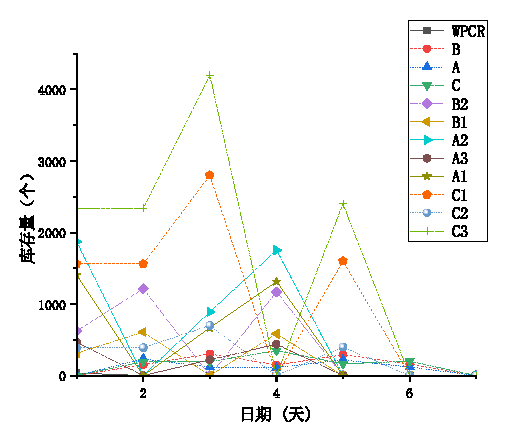
\includegraphics{Image/问题二库存.eps}
	\caption{问题二库存}\label{问题二库存}
\end{figure}
% subsection 生产方案展示 (end)
% section 工厂生产计划扩展 (end)